\documentclass{article}

\usepackage{tikz}
\usetikzlibrary{automata,positioning}
\begin{document}

\centering
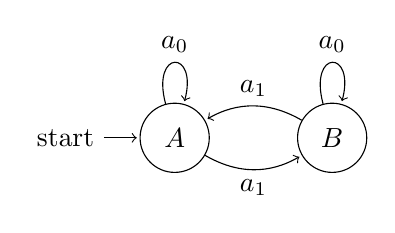
\begin{tikzpicture}[shorten >=1pt,node distance=2cm,on grid,auto] 
   \node[state,initial] (A)   {$A$}; 
   \node[state](B) [right=of A] {$B$};
    \path[->] 
    (A) edge [loop above] node {$a_0$} (A)
    (B) edge [loop above] node {$a_0$} (B)
    (A) edge[bend right]  node[pos=0.5, sloped, below]  {$a_1$} (B)
    (B) edge[bend right]  node[pos=0.5, sloped, above]   {$a_1$} (A);
\end{tikzpicture}

\vspace*{2cm}

\begin{table}[h]
\centering
\begin{tabular}{|l|l|l|}
\hline
  & \multicolumn{1}{c|}{A} & B    \\ \hline
A & $a_0$                   & $a_1$ \\ \hline
B & $a_1$                   & $a_0$ \\ \hline
\end{tabular}
\caption{Aktionen in der Umgebung}
\end{table}

\vspace*{2cm}
\centering
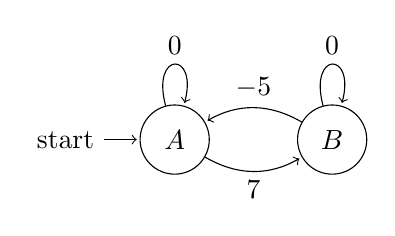
\begin{tikzpicture}[shorten >=1pt,node distance=2cm,on grid,auto] 
   \node[state,initial] (A)   {$A$}; 
   \node[state](B) [right=of A] {$B$};
    \path[->] 
    (A) edge [loop above] node {$0$} (A)
    (B) edge [loop above] node {$0$} (B)
    (A) edge[bend right]  node[pos=0.5, sloped, below]  {$7$} (B)
    (B) edge[bend right]  node[pos=0.5, sloped, above]   {$-5$} (A);
\end{tikzpicture}

\vspace*{2cm}

\begin{table}[h]
\centering
\begin{tabular}{|l|l|l|}
\hline
  & \multicolumn{1}{c|}{A} & B   \\ \hline
A & 0.1                    & 0.9 \\ \hline
B & 0.9                    & 0.1 \\ \hline
\end{tabular}
\caption{Transitions Matrix mit Wahrscheinlichkeiten}
\end{table}

\vspace*{2cm}

\end{document}  